\documentclass[a4paper]{article}
\usepackage[T1]{fontenc}
\usepackage{times,mathptm}
\usepackage[scaled=0.80]{beramono}
\usepackage{rascal}
\usepackage{highlight}
\usepackage{hyperref}
\usepackage{url}
\usepackage{epsfig}
\usepackage{float}

\def\source#1#2{\href{http://svn.rascal-mpl.org/lwc/trunk/lwc11/src/#1}{#2}}
\floatstyle{ruled}
\newfloat{listing}{htbp}{lol}
\floatname{listing}{Listing}

\begin{document}

\title{Language Workbench Comparison 2011 --- \Rascal}
\author{Tijs van der Storm\\
\textsl{CWI, Amsterdam}\\
\texttt{storm@cwi.nl}}
\maketitle

\section*{Introduction to \Rascal}

\begin{itemize}
\item Source-to-source
\item Modular syntax definition
\item Function programming language (immutable data)
\item IDE integration with Eclipse throug IMP
\end{itemize}

\section*{Phase 0}

\subsection*{Task 0.1: A Language for Entities}

\begin{listing}
\begin{rascal}
import lang::entities::syntax::Layout;
import lang::entities::syntax::Ident;
import lang::entities::syntax::Types;

start syntax Entities
    = entities: Entity* entities;

syntax Entity 
    = @Foldable entity: "entity" Name name "{" Field* "}";

syntax Field 
    = field: Type Ident name;
\end{rascal}
\caption{\source{lang/entities/syntax}{Syntax definition of
  entities.}}
\end{listing}

\begin{figure}
\begin{center}
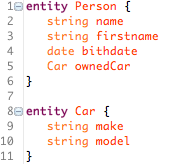
\epsfig{file=entities,width=0.3\linewidth}
\end{center}
\caption{Screenshot of an Eclipse editor showing highlighted entities\label{FIG:entities}}
\end{figure}

\begin{listing}
\begin{rascal}
data Entities = entities(list[Entity] entities);
    
data Entity = entity(Name name, list[Field] fields);
    
data Field = field(Type \type, str name);

data Type = primitive(PrimitiveType primitive)
          | reference(Name name);
    
data Name = name(str name);

data PrimitiveType = string() | date() | integer() | boolean();
\end{rascal}
\caption{\source{lang/entities/ast/Entities.rsc}{Abstract syntax of
    entities.}}
\end{listing}


\subsection*{Task 0.2: Code Generation To Java}

\begin{listing}
\begin{rascal}
public str entity2java(Entity e) {
    return "public class <e.name.name> {
        '<for (f <- e.fields) {>
        '  <field2java(f)>
        '<}>
        '}";
}

public str field2java(field(typ, n)) {
    <t, cn> = <type2java(typ), capitalize(n)>;
    return "private <t> <n>;
           'public <t> get<cn>() {
           '    return this.<n>;
           '}
           'public void set<cn>(<t> <n>) {
           '    this.<n> = <n>;
           '}";
}
\end{rascal}
\caption{\source{lang/entities/compile/Entities2Java.rsc}{Functions to
    generate Java classes.}}
\end{listing}

\subsection*{Task 0.3: Constraint Checking}

\begin{listing}
\begin{rascal}
public list[Message] check(Entities es) {
    defs = {};
    errors = for (e <- es.entities) {
        if (e.name in defs) {
            append error("Redeclared entity", e@location);
        }
        defs += {e.name};
    }
    return ( errors | it + checkEntity(e, defs) | e <- es.entities );
}

public list[Message] checkEntity(Entity e, set[Name] defs) {
    fs = {};
    return for (f <- e.fields) {
        if (f.name in fs) {
            append error("Duplicate field", f@location);
        }
        if (reference(Name n) := f.\type, n notin defs) {
            append error("Undefined entity type", n@location);
        }
        fs += {f.name};
    }
}
\end{rascal}
\caption{\source{lang/entities/check/Entities.rsc}{Functions to check
    entities for errors.}}
\end{listing}

\subsection*{Task 0.4: Breaking Down Models}

\begin{listing}
\begin{rascal}
public Entities merge(loc files...) {
    return merge({ parse(f) | f <- files });
}

public Entities merge(set[Entities] ess) {
    return entities(( [] | it + es.entities | es <- ess ));
}
\end{rascal}
\caption{\source{lang/entities/utils/Merge.rsc}{Utility functions to
    merge multiple entity files into a single set of entities}}
\end{listing}



\section{Phase 1}

\subsection*{Task 1.1: a Language for Instances}

\begin{listing}
\begin{rascal}
import lang::entities::syntax::Ident;
import lang::entities::syntax::Layout;

start syntax Instances = instances: Instance* instances;

syntax Instance
    = @Foldable instance: Name entity Name name "=" "{" Assign* "}";
    
syntax Assign = assign: Ident name "=" Value;
    
syntax Value 
    = date: Int "." Int "." Int
    | string: Str
    | integer: Int
    | reference: Name name;
    
syntax Int = lex [0-9]+ # [0-9];

syntax Str = lex [\"] StrChar* [\"];

syntax StrChar = lex ![\\\"] | lex [\\][\"\\];
\end{rascal}
\caption{\source{lang/instances/syntax/Instances.rsc}{Syntax definition for the
    instances language}}\label{LST:instances}
\end{listing}

\subsection*{Task 1.2: Type Checking Instances}

assume we have entities to check against; nb actual impl, uses require

\begin{listing}
\begin{rascal}
public list[Message] check(Instances is, Entities es) {
    edefs = ( e.name: e | e <- es.entities );
    idefs = ();
    errors = for (i <- is.instances) {
        if (i.\type notin edefs) {
              append error("Undefined type", i@location);
        }
        if (i.name in idefs) {
            append error("Duplicate instance", i@location);
        }
        idefs[i.name] = i.\type;
    }
    return ( errors | it + check(i, idefs, edefs[idefs[i.name]]) 
                    | i <- is.instances, i.\type in edefs );
}

public list[Message] check(Instance i, map[Name, Name] idefs, Entity e) {
    fdefs = ( f.name: f.\type | f <- e.fields );
    
    list[Message] errors = 
        [ error("Undefined field", a@location) 
            | a <- i.assigns, a.name notin fdefs ]
    
        + [ error("Undefined instance", a@location)
            | a <- i.assigns,  reference(Name n) := a.\value, n notin idefs ]
                
        + [ error("Missing field <n>", i@location) 
            | n <- domain(fdefs) - { a.name | a <- i.assigns } ];
    
    return ( errors | it + checkTypes(a, fdefs[a.name], a.\value, idefs) 
                    | a <- i.assigns, a.name in fdefs );
}
\end{rascal}
\caption{\source{lang/instances/check/Instances.rsc}{Type checking of
    instances against entity definitions.}\label{LST:checkInstances}}
\end{listing}


\subsection*{Task 1.3: Model-to-Model Transformation}

\begin{listing}
\begin{rascal}
data Database = database(list[Table] tables);

data Table = table(str name, list[Column] columns);

data Column 
     = column(str name, ColumnType \type, list[Constraint] constraints);

data ColumnType = integer() | boolean() | varchar() | date() | text();
    
data Constraint 
     = unique() | key() | notNull() | references(str table, str column);
\end{rascal}
\caption{\source{lang/database/ast/Database.rsc}{Abstract syntax for
    relational databases}}\label{LST:database}
\end{listing}

\begin{listing}
\begin{rascal}
private str KEY = "_id";

public Database entities2database(Entities es) {
    return database([ entity2table(e) | e <- es.entities ]);
}

public Table entity2table(Entity e) {
    cols = [column(KEY, integer(), [key()])] 
         + [ field2column(f) | f <- e.fields ];
    return table(e.name.name, cols); 
}

public Column field2column(Field f) {
    t = type2columnType(f.\type);
    cs = [];
    if (reference(name(e)) := f.\type) {
        cs = [references(e, KEY)];
    }
    return column(f.name, t, cs);
}
\end{rascal}
\caption{\source{lang/entities/transform/Entities2Database.rsc}{Transforming
  entity models to a database model.}}\label{LST:entities2database}
\end{listing}

\subsection*{Task 1.4: Namespaces}

Note reuse of grammar Entities. Extension of the name non-terminal.

\begin{listing}
\begin{rascal}
import lang::entities::syntax::Entities;
import lang::entities::syntax::Layout;
import lang::entities::syntax::Types;
import lang::entities::syntax::Ident;

start syntax Package
    = package: "package" Ident name "{" 
                       Import* imports 
                       Entities entities 
                "}";

syntax Import = imp: "import" Ident name;

syntax Name = qualified: Ident "." Ident;
\end{rascal}
\caption{\source{lang/packages/syntax/Packages}{Extension of the
    entities language to support name spaces
    (packages).}\label{LST:packages}} 
\end{listing}

\subsubsection{Loading, Resolving, Checking}
Overview of the rest
- loading: WorkingSet
- checking: check name collisions etc.
- run resolver: substitute names for qualified names (= source-to-source)
- run default entities checker after resolution


\subsubsection{Java Code Generation}

Assume pkg has been resolved.

\begin{listing}
\begin{rascal}
import lang::packages::ast::Packages;
extend lang::entities::compile::Entities2Java;

public str package2java(Package pkg) {
    return "package <pkg.name>;
           '<for (i <- pkg.imports) {>
           'import <i.name>.*;
           '<}>
           '<intercalate("\n", entities2java(pkg.entities))>";
}

public str type2java(qualified(str pkg, str name)) = "<pkg>.<name>";
\end{rascal}
\caption{\source{lang/packages/compile/Package2Java.rsc}{Extension of
    the entities code generator to support
    packages}\label{LST:package2java}}
\end{listing}



\subsection*{Task 1.5: Integrating Manually Written Code}

Show both extensions at once. Could be separate.

\begin{listing}
\begin{rascal}
import lang::entities::syntax::Layout;
import lang::entities::syntax::Ident;
import lang::entities::syntax::Types;
import lang::entities::syntax::Entities;

syntax Field 
    = derived: Type Ident "=" Expression
    | annotated: Annotation Type Ident ;
    
syntax Annotation = annotation: "@" Ident "(" String ")"; 
\end{rascal}
\caption{\source{lang/derived/syntax/Derived.rsc}{Extending the
    entities language to support computed
    attributes.}\label{LST:derived}}
\end{listing}

\begin{listing}
\begin{rascal}
extend lang::entities::compile::Entities2Java;
import lang::derived::ast::Derived;

public str field2java(derived(t, n, exp)) {
    return getter(t, n, exp2java(ex));
}

public str field2java(annotated(a, t, n)) {
    method = substring(a.string, 1, size(a.string) - 1);
    return getter(t, n, "<method>(this)");
}

private str getter(Type t, str n, value exp) {
    <tn, cn> = <type2java(t), capitalize(n)>;
    return "public <tn> get<cn>() {
           '    return <exp>;
           '}";
}
\end{rascal}
\caption{\source{lang/derived/compile/Derived2Java.rsc}{Extending the
    Java generator to support computed
    attributes.}\label{LST:derived2java}}
\end{listing}



\subsection*{Task 1.6: Multiple Generators}

Example: entities to XML

\begin{listing}
\begin{rascal}
import XMLDOM;

public Node entities2xml(Entities es) {
    return document(element(none(), "entities", 
       [ entity2element(e) | e <- es.entities ]));
}

public Node entity2element(Entity e) {
    a = attribute(none(), "name", e.name.name);
    return element(none(), "entity", 
       [a, [ field2element(f) | f <- e.fields ]]); 
}

public Node field2element(Field f) {
    attrs = [attribute(none(), "name", f.name)];
    if (primitive(t) := f.\type) {
        attrs += [attribute(none(), "type", getName(t))];
    }
    else {
        attrs += [attribute(none(), "type", "ref"),
                    attribute(none(), "references", f.\type.name.name)];
    }
    return element(none(), "field", attrs); 
}
\end{rascal}
\caption{\source{lang/entities/compile/Derived2XML.rsc}{Generate XML
    for entities.}\label{LST:entities2xml}}
\end{listing}

\section*{Phase 2: Non-Functional}

- Source code based: collaborating through VCS is automatic.

- Modular syntax def allows a ``previous'' grammar to co-exist with
the new one. It is natural to define ``upgrade'' transformations from
old DSL code to new stuff.


\section*{Phase 3: Free-style}

Concrete syntax matching (example: Refactoring?) Could have written
all the tasks above, without abstract syntax.

IDE integration

\end{document}